\documentclass[11pt]{article} 
\usepackage{geometry}
\geometry{a4paper}
\usepackage{graphicx}
\usepackage{hyperref}
\usepackage{amsmath}

\begin{document}

\begin{titlepage}
 
\title{\huge{\textbf{Fading Signal Propagation Model}}}
\date{}
\author{}
\maketitle
\vspace{4 cm}
\center{\textbf{\huge{Manual v3}}} 
\vspace{4 cm}
\center{\small{Daniel Rovera, }}
\center{Team Computational Systems Biology of Cancer \\ Institut Curie \\ 26, rue d'Ulm \\ 75005 Paris}

\end{titlepage}

\tableofcontents

\newpage
This application of Cytoscape 3.x provides functions of visualizing and computing influence spreading to a directed network where edges are activation on inhibition. This application is based on a simple model described in ~\ref{FadeModel}).

\section{Utils\&Analysis}

\subsection{Preselect Sources and Targets}
Preselect in dialogs nodes as sources or as targets. So, these nodes are selected, when opening list boxes. The node attribute PRESELECTED is set to 1 if source, to 2 if target, to 3 if both target and source. If Not preselected it is set to 0. It can be directly imported as node attribute by Cytoscape.

\subsection{Select Sub-network from Sources to Targets}
This function selects nodes and edges in the directed network between a list of sources and a list of targets.  Loops are included in the selection.

\subsection{Display SCC in Attribute}
Display in node attribute if the node is in a SCC group or not in SCC. The SCC group are numbered (SCC: strong connected components).

\subsection{Display Signed Distances}
After selecting sources and targets, display the number of paths from sources to targets signed by weights according to the path mode (the parameter "reach" is only necessary for multi path mode).

\subsection{List Opened Edges MultiPath Only}
Only usable in multi path mode. List back edges which are opened to avoid loop and allow multi path computing.


\section{Parameters\&Calibration}

\subsection{Update Weight Attribute}
A weight of influence as edge attribute must be affected to every edge. This dialog updates the weight attribute by 
\begin{itemize}
\item selecting the attribute containing the edge influence,
\item affecting its values to activation (weight=+1) and inhibition (weight=-1).
\end{itemize}
3 possible values for the attribute. Generally, the attribute is "interaction" and the values "activation" or "inhibition". Be careful of lower-case and upper-case (see~\ref{Weight_Attribute_Dialog}).\\
The edge attribute "WEIGHT" contains those value which can be input directly by Cytoscape.

% change graphics 
\begin{figure}
\centering
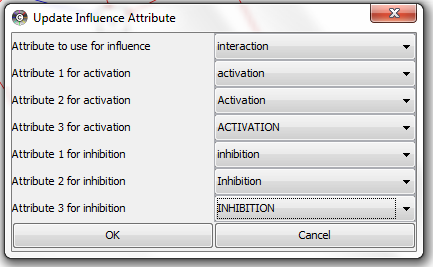
\includegraphics[width=0.7\textwidth]{graphics/Weight_Attribute_Dialog}
\caption{Dialog updating weight attribute from an other attribute}
\label{Weight_Attribute_Dialog}
\end{figure}

\subsection{Select Mono or Multi Path Mode}
This function selects the type of exploring mode: multi path or mono path.

\subsection{Input Reach Parameter}
Input the number of paths beyond which the influence is insignificant, less than 5\%. It is a floating point number, not necessary integer.

\subsection{Input Score Threshold}
Input the threshold used to round influence values and, so, to compute kappa. 

\subsection{Network and Parameter Features}
Display in a text box: network, size of network, reach parameter, min, max, mean and standard deviation influence, computed by excluding not connected nodes. It a recapitulation of parameters and their effect on influence matrix.

\section{Numeric Influence}

\subsection{Display Influence Array For Visualizing}
The influence matrix is displayed in a text box which can be copied in the clipboard and paste in a spreadsheet, sources in columns, targets in rows, names in alphabetical order. Parameters and option are in window title. The format is: 3 digits after point for numbers and "nc" = not connected.\\
Same dialog as "Select Sub-network from Sources to Targets". Preselected sources and targets can be used.  For all nodes as sources or targets: select the first node and type shift+control+end.

\subsection{Display Influence Array For Computing}
Idem but all values are numeric with all possible digits. Less readable but better adapted for computing.

\subsection{Display Influence As List}
Same result than Display Influence Array As Text For Computing, but as a list between every both nodes.

\subsection{Influence by Active Nodes as Attribute}
Activity levels of nodes are input in an attribute "ACTIV\_IN". The result of the multiplication of influence matrix by activity level input is "ACTIV\_OUT" attribute.

\subsection{Display Influence Array Between Subnetworks}
Display influence array for computing between sub-networks selected in network panel. The influence between sub-networks is the sum of influence of nodes inside sub-networks.\\
The sub-networks must be extracted from a reference network which must be input and which carries the parameters in its attributes. Pieces of incoherence between the sub-networks and the reference network are also displayed in the text box.

\section{Graphic Influence}
\subsection{Display Influence Array as Blue White Red Paved Window}
Same computing as "Display Influence Array For ...", but the results are   
\begin{itemize}
\item as a colored paved window, activated in red, inhibited in blue, light to dark according to the value, not connected in white (see~\ref{paved_window}).
\item when selecting blocs and clicking, influences between nodes in selected blocs are displayed in a text window.
\end{itemize}

\subsection{Display Influence Array as Green Black Red Paved Window}
Idem with activated in red, inhibited in green, light to dark according to the value, not connected in black.

\begin{figure}
\centering
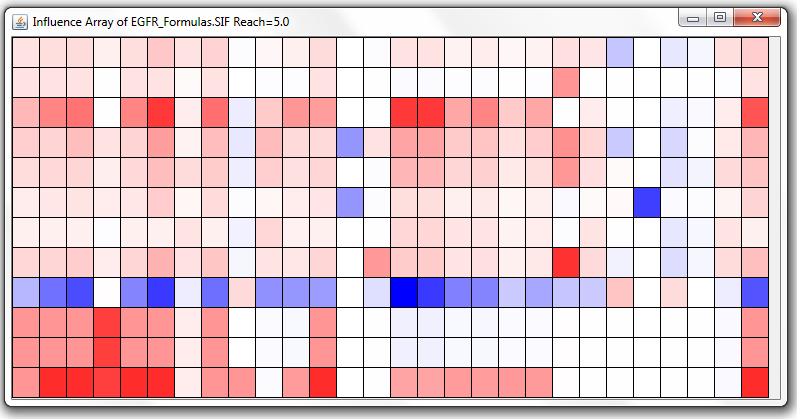
\includegraphics[width=1.0\textwidth]{graphics/paved_window}
\caption{Window paved by the level of influence between species}
\label{paved_window}
\end{figure}

\section{Reach Area}

\subsection{Display Influence Reach Area in Array}
Computing as "Display Influence Array for Computing" with all weights=1. Useful to appreciate the absolute level of influence by a specie to other species.

\subsection{Influence Reach Area as Attribute}
Computing from selected nodes with all weights=1. Absolute influence levels are put in attribute "INFLUENCE\_AREA\_N" where N keeps every successive results. Start nodes and options must be noted manually. Useful to visualize the influence of a group of species.

\section{Comparing to Measures}

\subsection{Compute Score of Data Sets }
Data must be input as node attributes:
\begin{itemize}
\item Activity levels of source nodes as input, attribute "INPUT\_\_SETidentifier" (2 underscores), identifier may be a number or a word, 
\item Expected activity levels of target nodes as output aim, attribute "OUTPUT\_AIMidentifier", identifier matches input with output.
\end{itemize}
The result is a tabulated text including size of data sets, number of maching output (with threshold) and Cohen's kappa coefficient (see~\ref{Score_Of_Data_Sets} and, about definition see~\ref{FadeModel}).
If level \textless -threshold, node is taken as inhibited. If level \textgreater +threshold, node is taken as activated.

\begin{figure}
\centering
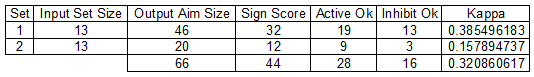
\includegraphics[width=1.0\textwidth]{graphics/Score_Of_Data_Sets}
\caption{Score of data sets formatted in a spreadsheet}
\label{Score_Of_Data_Sets}
\end{figure}

\subsection{Test Score by Reversing Sign Weight }
Test if reversing sign weight of every edge improves kappa, display list of edges sorted by decreasing kappa.

\subsection{Test Score by Canceling Weight }
Test if canceling sign weight of every edge improves kappa, display list of edges sorted by decreasing kappa. No change in structure network.

\section{Description of Fading Signal Propagation Model}\label{FadeModel}
\subsection{Computing at nodes and along edges}
The network for this model is a directed graph where edges are weighted: weight = +1 if activation and weight = -1 if inhibition. Any real value of weight can be used, but the accuracy of this model casts a doubt about this way.\\
The model is based on fading propagation of the biological signal. The fading effect is simply translated as multiplying edge weights by a global positive factor \textquotedblleft fade\textquotedblright (less than 1) along every edge.  Fade is translated to a number of paths "reach", which is input, by  $fade^{reach}$ = 5\%.
\\Influence on a node is the sum of influences from upstream nodes by incoming edges. This model is the simplest which respect the transitivity by addition of the path lengths as:\\
$activity(at\ length1,activity(at\ length2,start\ active\ node)=\\\hspace*{2em}activity(at\ length1+length2, start\ active\ node)$\\
More precisely, when going all over the network, the recurrence from every root and every edge (source, target) from the root is:
\begin{itemize}
\item $all\_influence = 0$
\item $influence (root, root) = 1$
\item $influence (root, target)= influence (root, target) +\\influence (root, source) * fade * weight (source, target)$
\end{itemize}
The structure of the network is described by an adjacency list matching every node to lists of adjacent edges. Going over the network can be done by two exploring mode:
\begin{enumerate}
\item mono path: exploration by by breadth first search ends when a node already reached is found, every edge edge is counted once ; 
\item multi path: loops are opened as far as possible from source by depth first search (back edges), after all paths are explored in order of distances from the source, the exploration stops at 2*reach  ;
\end{enumerate}
So,  the arrest of exploration at 2*reach keeps multi path process fast (error 0.25\%) while coping with forward feed path.
\subsection{Comparing to observations}
The result is a simple linear model as product of matrices:
\begin{itemize}
\item $[Activation\_level\_ output] = [Influence\_matrix] * [Activation\_level\_input]$
\end{itemize}
Activation\_level\_input can be the states of observed species in input of the network, values being generally:
\begin{itemize}
\item +1, if active
\item -1, if inactive
\item 0 if no observed
\end{itemize}
Activation\_level\_ output can be compared to observations of nodes in output of the network.\\
The computing performance allows to test on every edge weight=0 or weight=-weight to question the relevance of the network.\\
To compare model results and observations, only the number of matching signs are taken in a threshold near for computed values. As it exists an alternative, the pertinent indicator is Cohen's coefficient named kappa:\\
\hspace*{1cm}$kappa=(Po-Ph)/(1-Ph)$ \\
\hspace*{1cm}$Po$ is the relative observed agreement,\\
\hspace*{1cm}$Ph$ is the hypothetical probability of chance agreement.\\
The comparison can concern several sets of observations and, so, it gives a global appreciation of the network.

\end{document}
